\section{Cartograms with Rivers}
 {
  \begin{figure*}[tb!]
      \centering
      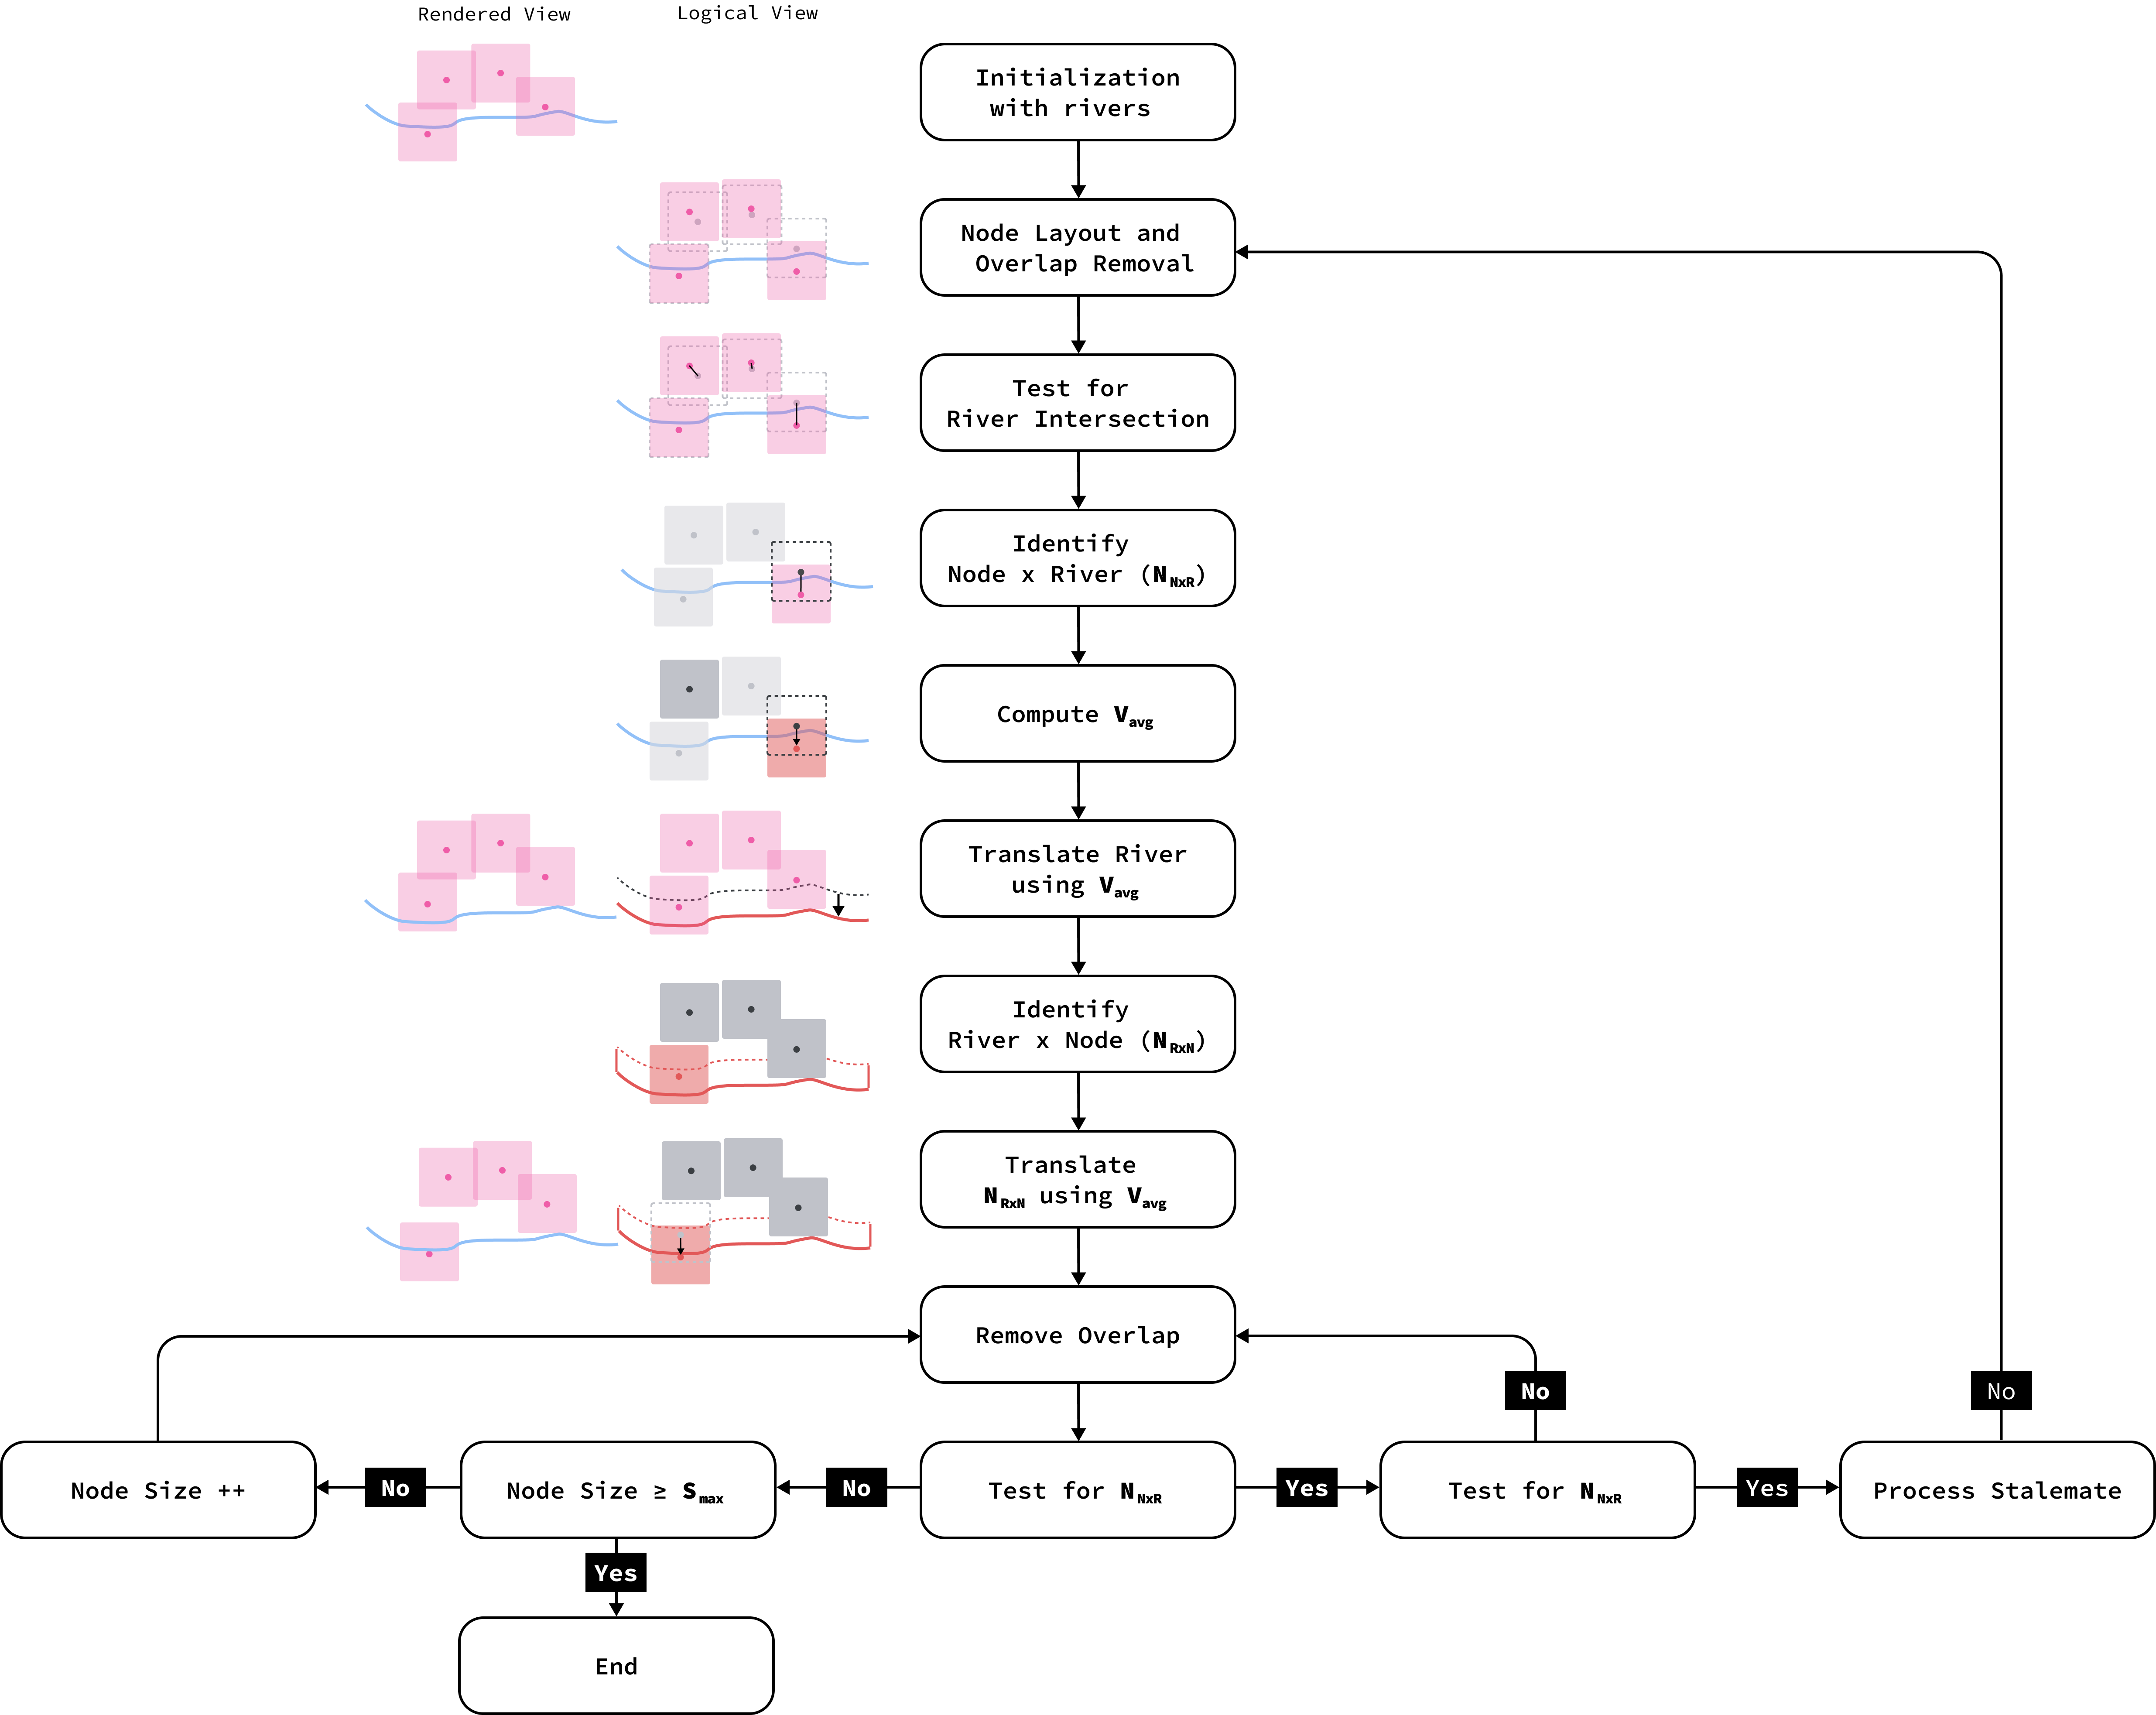
\includegraphics[width=\textwidth,height=\textheight,keepaspectratio]{figure/flowchart.png}
      \caption{A flowchart illustration of our layout algorithm. See \Cref{fig:flowchart-stalemate} for the logic of processing a stalemate. See also \Cref{alg:UpdateLayout} in \Cref{sec:{Cartograms with Rivers}} for more detail. For illustration purposes, we show the rendered views alongside the logical views representing the actual computation. \new{the notations here do not match those in Algorithms. Which ones to use?}}
      \label{fig:flowchart}
  \end{figure*}
 }

 {
  \begin{figure}[tb!]
      \centering
      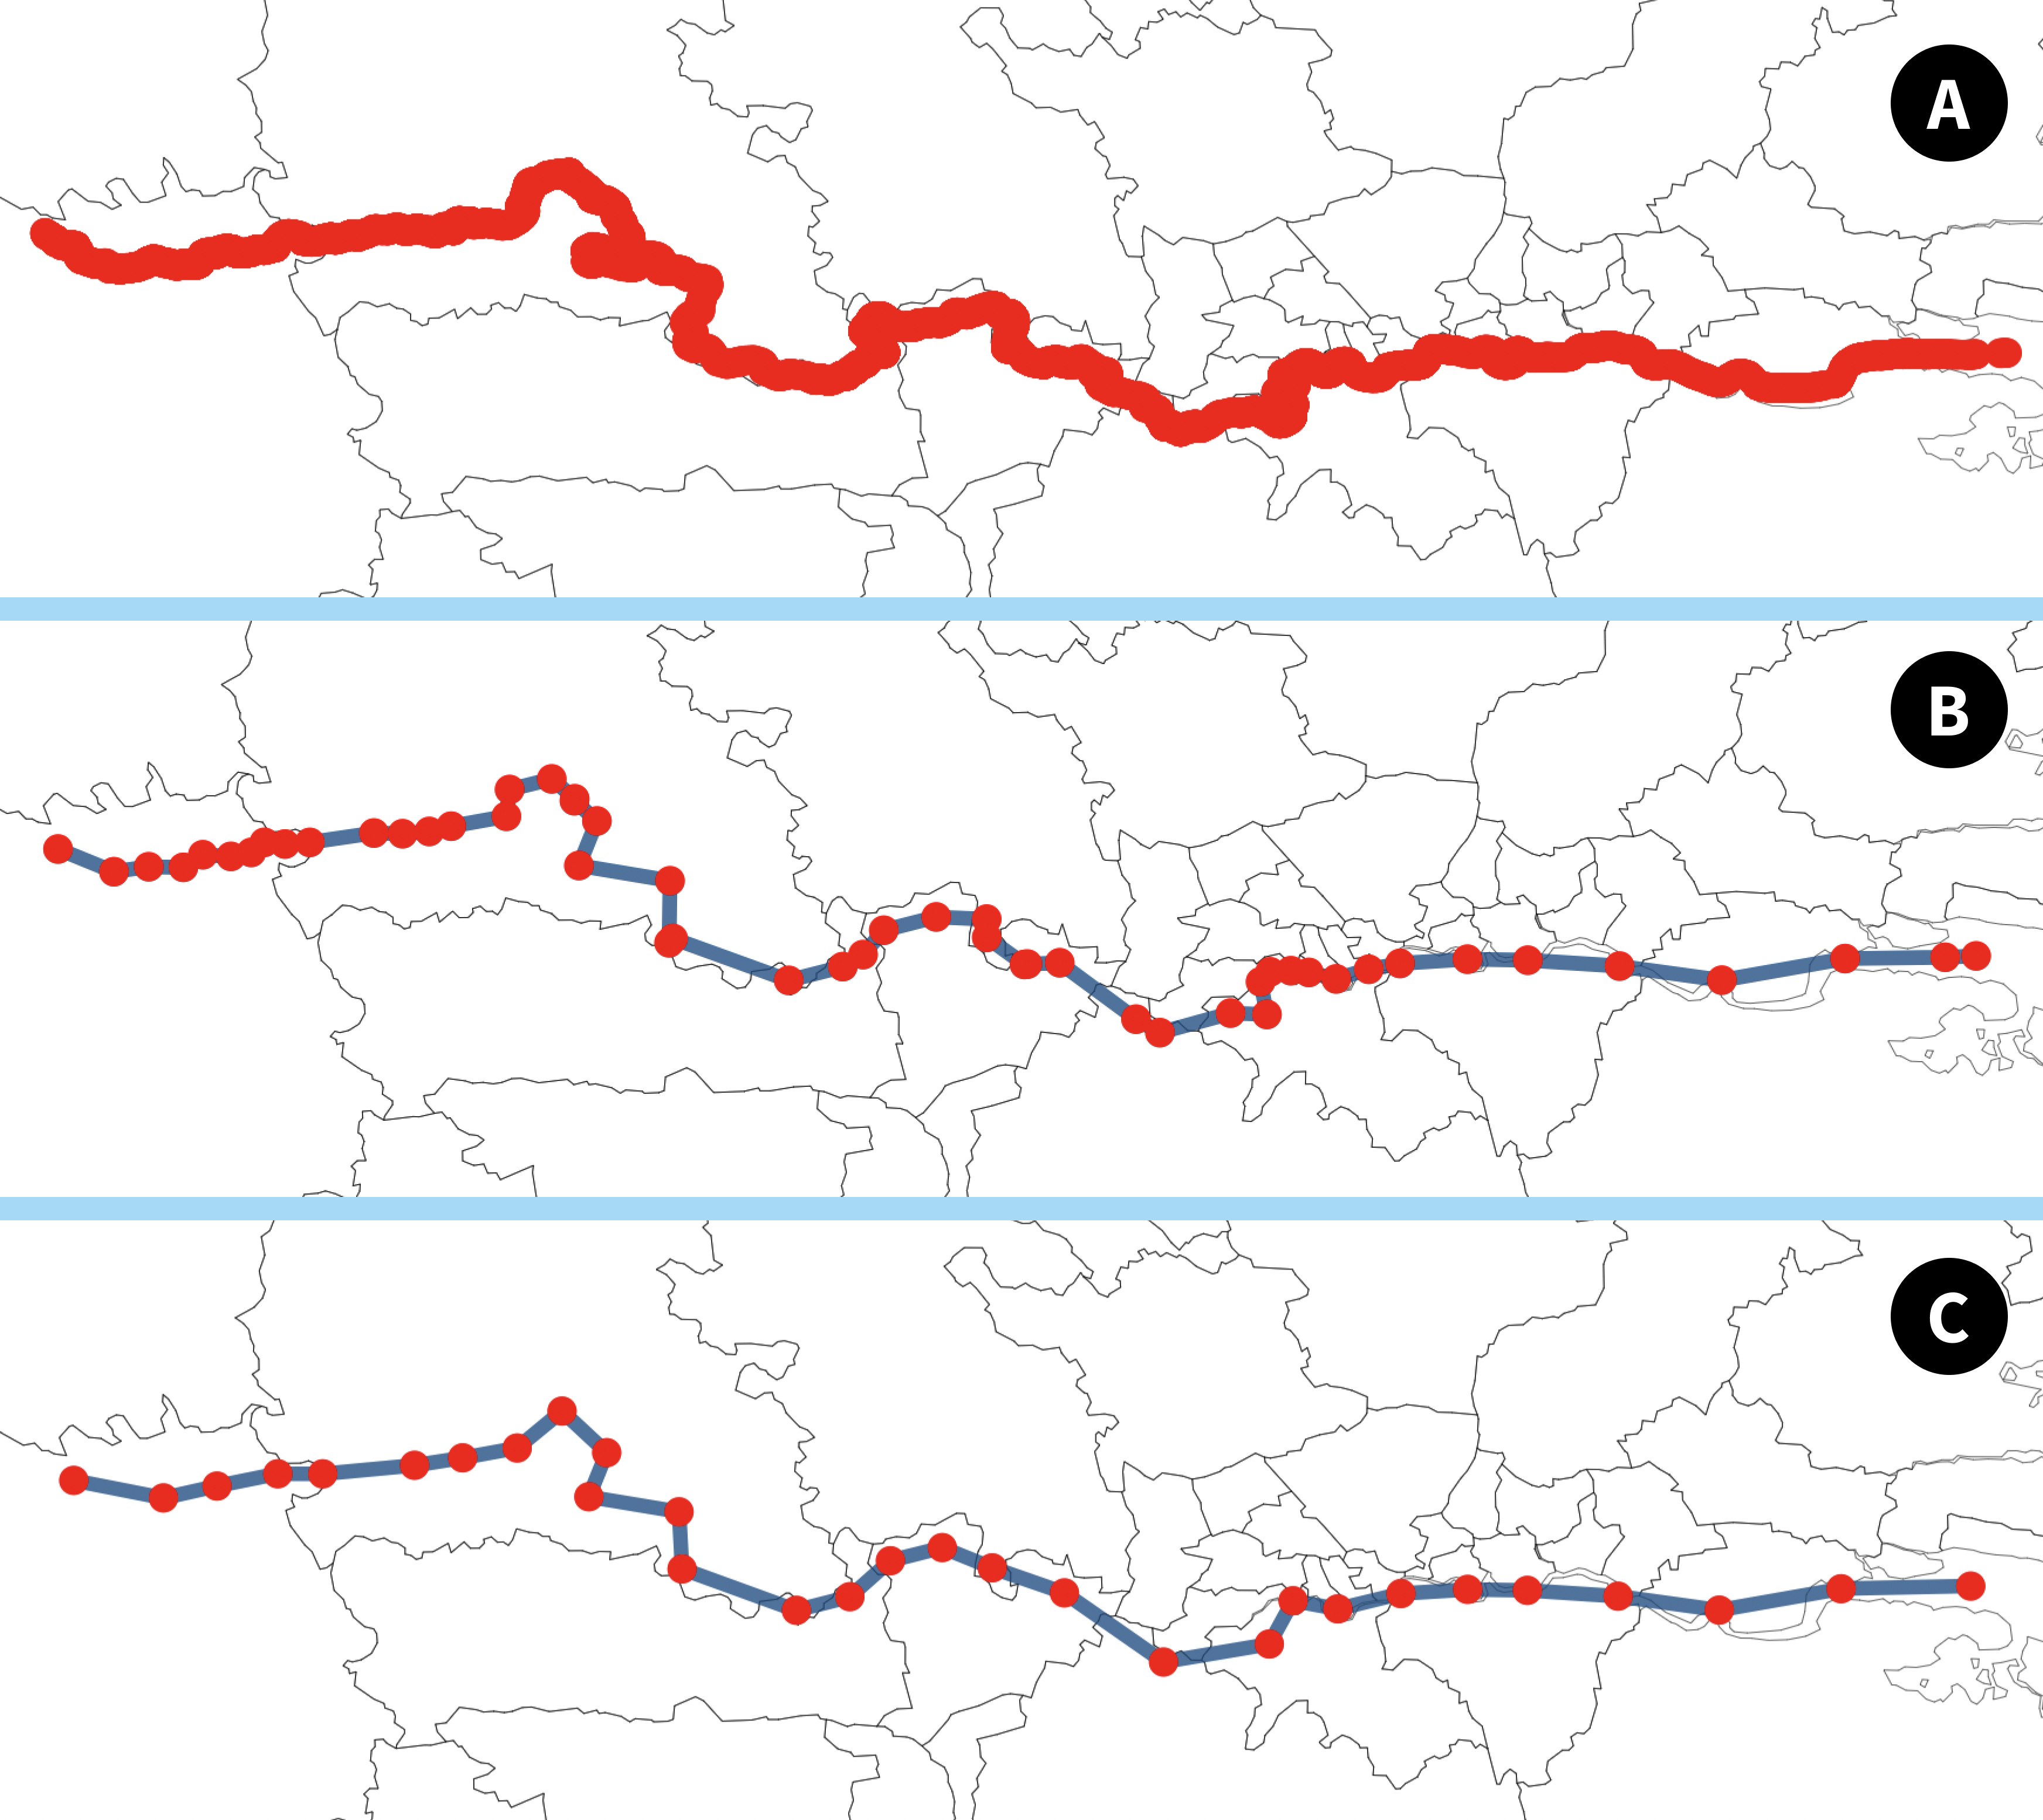
\includegraphics[width=0.7\columnwidth,keepaspectratio]{figure/river_resolution.png}
      \caption{The resolution of rivers can be dynamically adjusted by the user. (A) shows River Thames at its original resolution with 10,170 edges. (B) shows the river at a reduced resolution of 49 edges. We further smooth the river by removing 19 vertices in dense areas, as shown in (C). The reduced resolution preserves the majority of River Thames' original shape and improves the performance of our river intersection tests.}
      \label{fig:river resolution}
  \end{figure}
 }

 {
  \begin{figure}[tb!]
      \centering
      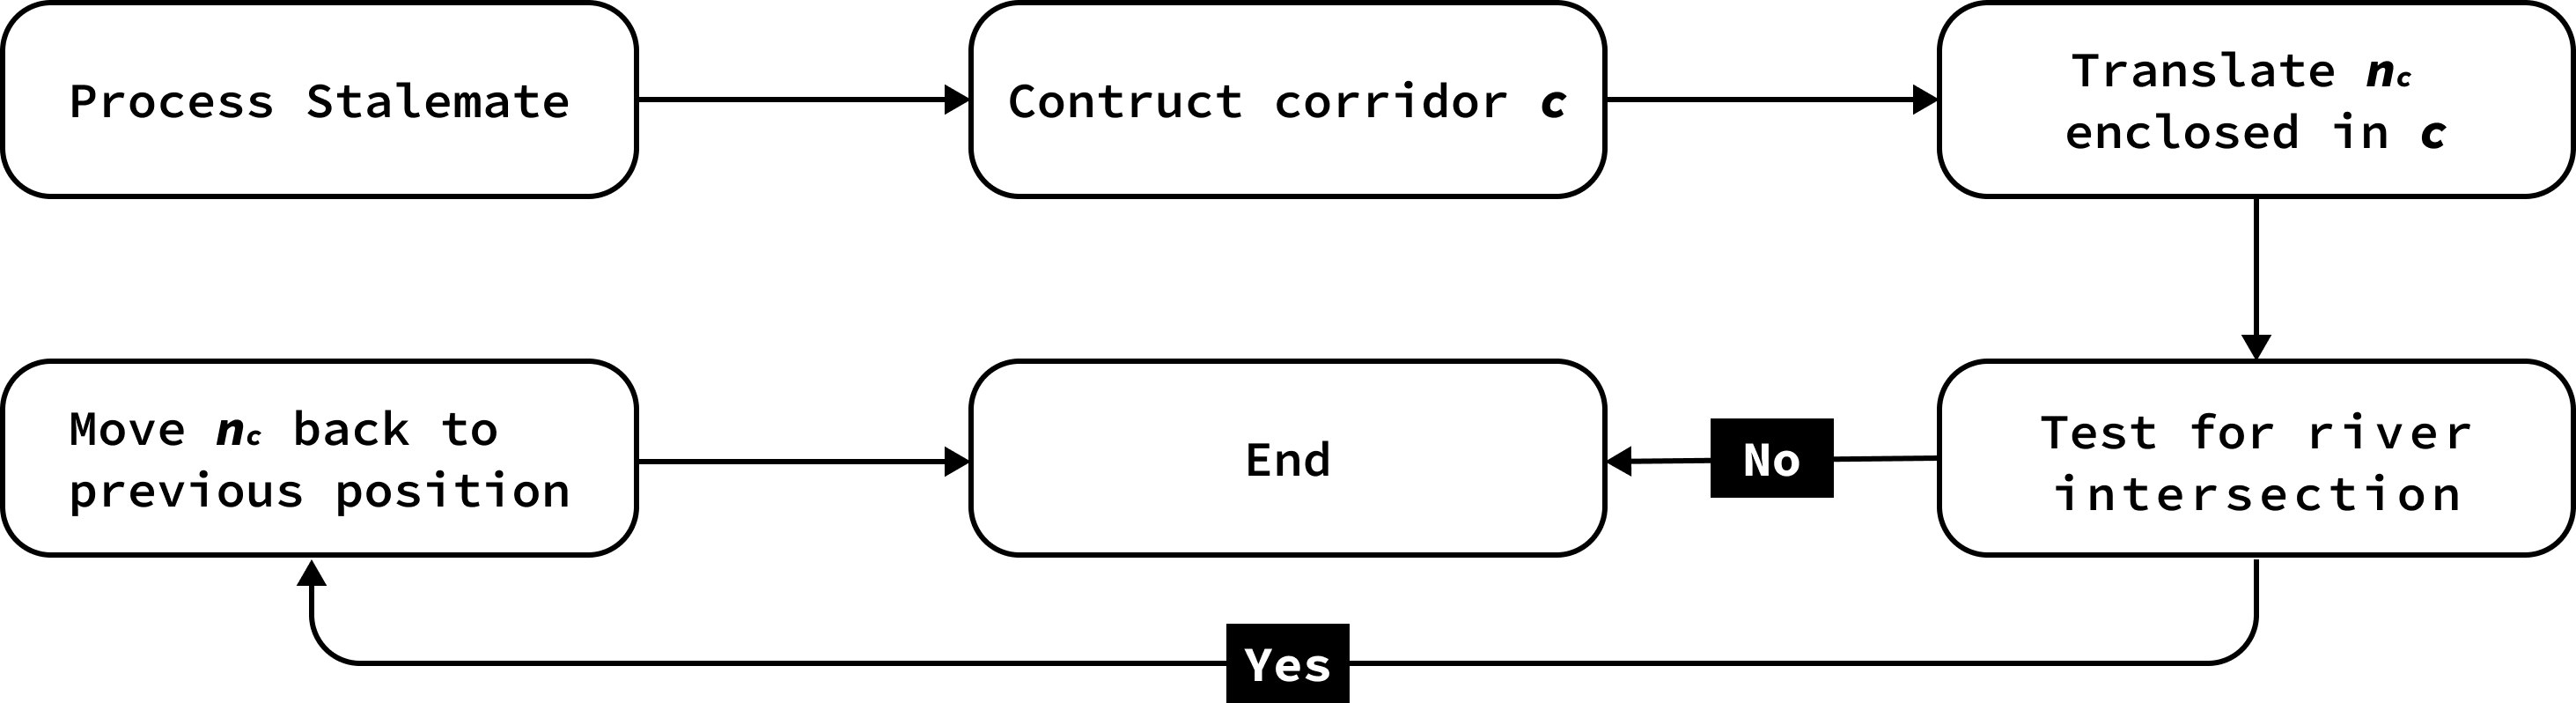
\includegraphics[width=\columnwidth,keepaspectratio]{figure/flowchart stalemate.png}
      \caption{A flowchart illustration of stalemate processing. See \Cref{subsec:{Detecting Stalemates}}, \Cref{fig:stalemate}, and \Cref{fig:corridor} for more detail.}
      \label{fig:flowchart-stalemate}
  \end{figure}
 }

\begin{algorithm}[tb!]
    \caption{Procedure to adjust river positions, remove node overlap and prevent nodes from crossing rivers. See \Cref{sec:{Cartograms with Rivers}}.}\label{alg:UpdateLayout}
    \textbf{Global variables:} \\
    $ \nodeList \gets $ a list of $ \node $ representing CCGs with the following properties: \\
    \-\hspace{1em}  $\nodeListCross \gets $ the number of $ \node $ in $ \nodeList $ that crosses a river \\
    $ \nodeSizeAvg \gets $ the average size of all nodes \\
    $ \nodeSizeMax \gets $ the maximum size of a node \\
    $ \stalemateMax \gets $ the maximum number of iterations indicating a stalemate \\

    \textbf{Local variables:} \\
    $ \node \gets $ a node is an object with the following properties: \\
    \-\hspace{1em} $ \node.x, \node.y, $ or $ \node(x,y) \gets $ the x and y coordinates of $ \node $ \\
    \-\hspace{1em} $ \nodeCross \gets $ the counter for river crosses for $ \node $ \\
    \-\hspace{1em} $ \nodePrevious \gets $ the previous position of $ \node $ \\
    \-\hspace{1em} $ \nodeFNOR \gets $ the translated position of $ \node $ \\

    \begin{algorithmic}[1]
        \Procedure{UpdateLayout}{}
        \While{$ \nodeSizeAvg < \nodeSizeMax $}
        \State $ \nodeListCross \gets 1 $ \Comment{Trigger the while loop}
        \While{$ \nodeListCross > 0 $}

        \State $ \nodeListCross \gets 0 $
        \State $ \nodeList \gets $ RemoveOverlap ($ \nodeList $)
        \State \Call{TranslateRiver}{$ \nodeList $}
        \State $\nodeListCross \gets $ \Call{TranslateNode}{$ \nodeList $}

        \EndWhile

        \State $ \nodeSize ++ $

        \EndWhile

        \EndProcedure
    \end{algorithmic}
\end{algorithm}


\Cref{alg:UpdateLayout} and \Cref{fig:flowchart} provide an overview of the cartogram layout process that includes rivers.

\bobgraph{Initialization with Rivers:} We first load and render the CCG geospatial boundaries. For each CCG we compute the centroid and represent it using a square node, $ \node $, with the initial size, $ \nodeSize $ of 1 pixel. We then load the river shapefiles and render the rivers. Since the vertices of the river in the shapefiles are not in sequential order, we first render the starting vertex, followed by the next nearest vertex. We do not need the original river resolution to incorporate them into cartograms. We reduce their resolution to match that of the cartogram nodes in order to facilitate node-river intersection tests. This rendering approach enables us to adjust the river resolution as shown in \Cref{fig:river resolution}. We further apply simplification by removing vertices that are too close to each other.


\bobgraph{Node Layout and Overlap Removal:} We first apply the Fast Node Overlap Removal (FNOR) algorithm that solves the Variable Placement with Separation Constraints (VPSC) problem \cite{dwyer2006fast} in order to remove overlap. We chose FNOR over other node overlap removal algorithms because FNOR is able to provide spread minimization and node movement minimization while maintaining a good level of global shape preservation \cite{chen2020Node}. Initialized with a pixel size of unity, we gradually increase the node size by one unit (proportional to its data) at a time to ensure smooth transitions. An increase in $ \nodeSize $ can cause the nodes to overlap. During overlap removal, we compute node trajectories (See \Cref{alg:check river intersection}) and translate nodes to their new position. Nodes that cross a river, denoted $ \nodeCross $, are translated back to their previous position. If a node oscillates across a river, we identify this as a stalemate. This procedure ends when 1) no node overlap is present; 2) no nodes cross a river. We then increase $ \nodeSize $ by one unit and repeat the algorithm until the average node size $ \nodeSizeAvg $ reaches the max node size $ \nodeSizeMax $. The gradual size increase process provides stability to the layout and helps minimize geographical error.

\begin{algorithm}[tb!]
    \caption{Procedure to translate node positions.}\label{alg:TranslateNode}

    \textbf{Input:} \\
    $ \nodeList \gets $ a list of $ \node $ representing CCGs \\

    \textbf{Output:} \\
    $ count \gets $ the number of river crossing nodes in the input \\

    \textbf{Global variables:} \\
    $ \stalemateMax \gets $ the maximum number of iterations indicating a stalemate \\

    \textbf{Local variables:} \\
    $ \node \gets $ a node is an object with the following properties: \\
    \-\hspace{1em} $ \node.x, \node.y, $ or $ \node(x,y) \gets $ the x and y coordinates of $ \node $ \\
    \-\hspace{1em} $ \nodeCross \gets $ the counter for river crosses for $ \node $ \\
    \-\hspace{1em} $ \nodePrevious \gets $ the previous position of $ \node $ \\
    \-\hspace{1em} $ \nodeFNOR \gets $ the translated position of $ \node $ \\

    \begin{algorithmic}[1]
        \Procedure{TranslateNode}{$ \nodeList $}
        \State $ count \gets 0 $
        \ForEach {$ \node \in \nodeList $}

        \If {$ \node(x,y) \neq \nodeFNOR(x,y) $}

        \State $ \node(x,y) \gets \nodeFNOR(x,y) $

        \If{ \Call{TestIntersection}{$ \nodeFNORLine $} $ = True $}
        \State $ \nodeCross ++ $
        \State $ count ++ $

        \If{$ \nodeCross < \stalemateMax $}
        \State \hskip-2em \Comment{Translate back to previous position}
        \State $ \node(x,y) \gets \nodePrevious(x,y) $

        \Else

        \State \Call{ProcessStalemate}{$ \node, \nodeFNOR $}
        \State $ \nodeCross \gets 0 $ \Comment{Reset counter}

        \EndIf

        \EndIf

        \EndIf

        \EndFor
        \State \Return{$ count $}
        \EndProcedure
    \end{algorithmic}
\end{algorithm}


\subsection{River Intersection Testing}

The logic for translating a node's position is detailed in \Cref{alg:TranslateNode}. When a node's position changes, we test if the node's trajectory intersects any segment of a river. See \Cref{alg:check river intersection}. A bounding box intersection test between the edge defined by node translation and river edges can be performed to reduce the number of edge intersection tests required. Using the intersection test, we identify all nodes that cross the river as a result of the initial FNOR algorithm. We label these nodes, $ \NxR $

\subsection{Translating Rivers}

For all nodes $ \NxR $ that cross a river, $ \river $, we compute an average vector $ \vectorAvg $ used to translate $ \river $. Whenever a node, $ \node $, crosses a river , we store a vector $ \nodeVectorNNn $ that points in the direction of the translation. We then use a heuristic to translate $ \river $ using the average vector of node intersection $ \vectorAvg = \sum_{i=1}^j \frac{\Vector{\node_i\node_{i_t}}}{j} $, where $ j $ is the number of nodes intersecting the river. This step intends to create space for the next iteration of node translation without crossing a river. The procedure for translating riers is provided by \Cref{alg:TranslateRiver} in the Appendix.

When a river is translated by $ \vectorAvg $, this can trigger a scenario where the nodes are crossed by a translated river, denoted $ \RxN $. As a heuristic we also translate these nodes by $ \vectorAvg $. The reasoning behind this is that $ \vectorAvg $ indicates which direction the river needs to be translated in order to create space for nodes that are too crowded together.

\subsection{Detecting Stalemates}

As the FNOR always attempts to produce an optimal node layout where node distribution and translation are minimized, a node's translation path can repeatedly intersect a river due to congestion, creating a stalemate situation, as shown in \Cref{fig:stalemate}. If a node is translated between two positions, $ \node $ and $ \nodeFNOR $, for $ \stalemateMax $ iterations (a user-adjustable parameter), we introduce a heuristic solution: constructing a corridor to alleviate the congestion. A corridor, $ \Corridor $, is a rectangle with a width of $ \CorridorWidth $ and a length of $ \CorridorLength $, formed by deriving two edges $ \EdgeParallelA $ and $ \EdgeParallelB $ such that $ \EdgeParallelA \parallel \EdgeParallelA \parallel \nodeLineNtNc $ (See \Cref{fig:corridor}C and D). All nodes enclosed by $ \Corridor $ are then translated by $ \nodeVectorTC $ to alleviate the congestion (See \Cref{fig:corridor}E). The procedure for constructing corridors is provided by \Cref{alg:derive corridor}.

    {
        \begin{figure}[tb!]
            \centering
            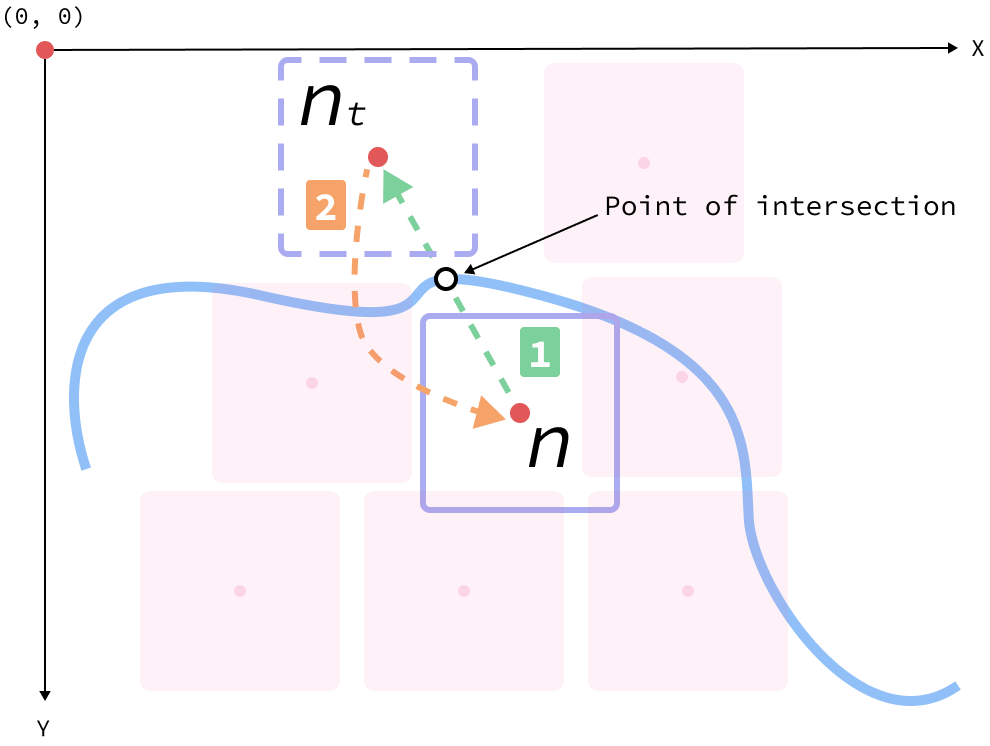
\includegraphics[width=\columnwidth,keepaspectratio]{figure/stalemate.png}
            \caption{A stalemate situation is when a node's translation path $ \nodeVectorCT $ (iteration 1) intersects a river $ \stalemateMax $ times. The node is translated back to its previous position (iteration 2). A stalemate often occurs when the area is congested and the node is unable to translate to a new position without intersecting a river.}
            \label{fig:stalemate}
        \end{figure}
    }

    {
        \begin{figure}[tb!]
            \centering
            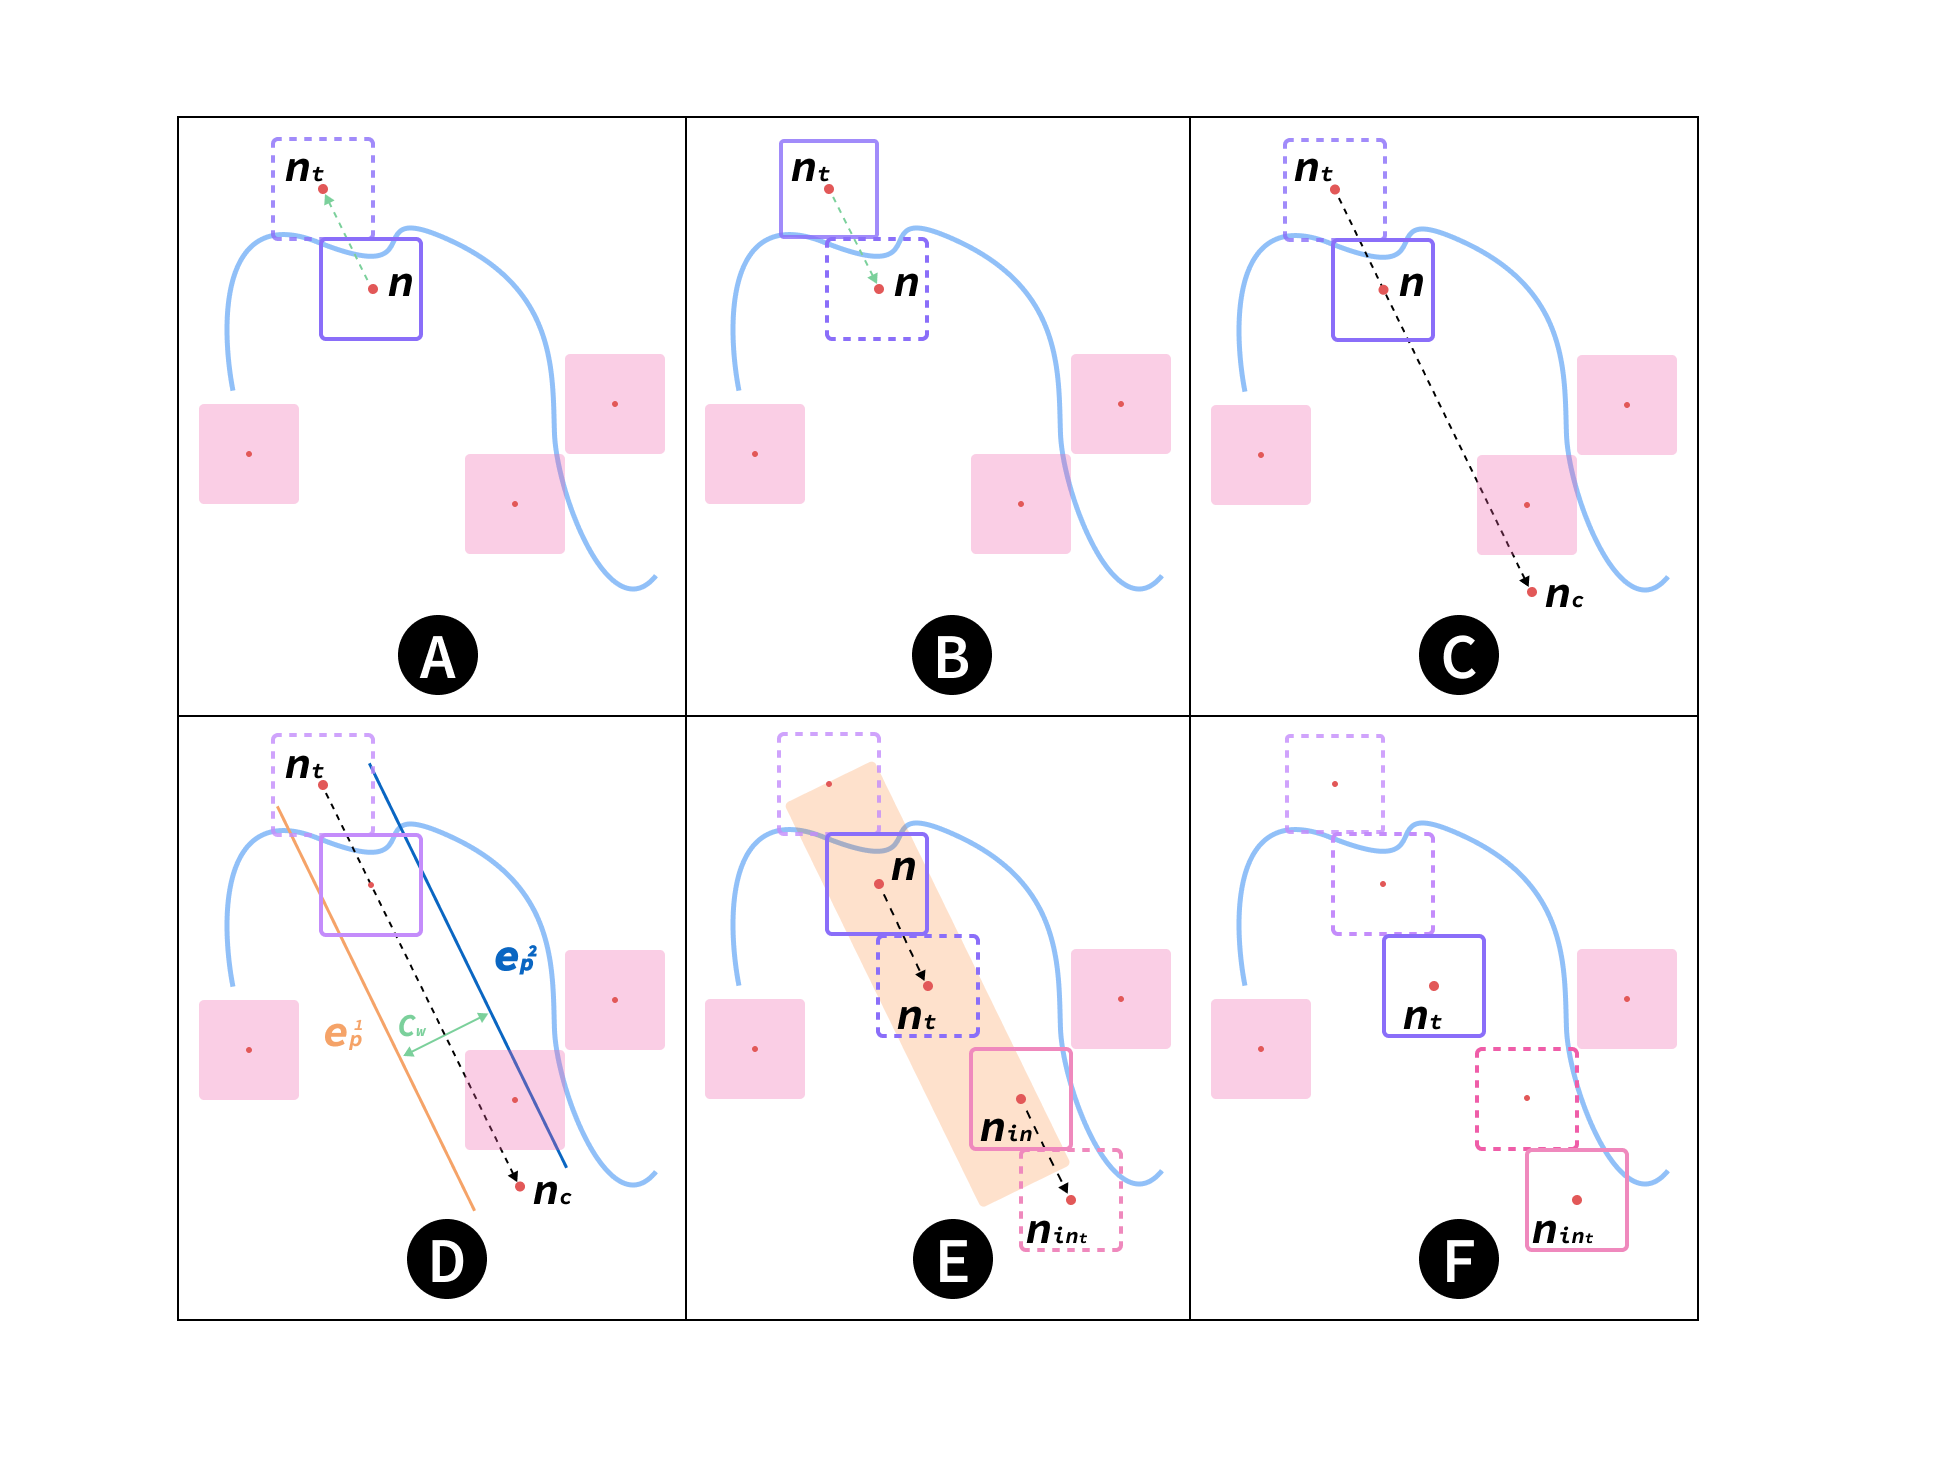
\includegraphics[width=\columnwidth,keepaspectratio]{figure/corridor.png}
            \caption{A stalemate occurs when a node's translation path $ \nodeVectorCT $ intersects a river for $ \stalemateMax $ times, as shown in (A). To address this, we derive a corridor (orange rectangle in (E)) based on $ \node $ and $ \nodeFNOR $. All nodes within the corridor are translated based on $ \nodeVectorTC $, such that $ \nodeVectorNNn = \nodeVectorNinNinn $. For clarity in the illustration, we place nodes sparsely in this figure.}
            \label{fig:corridor}
        \end{figure}
    }

% \begin{noindent}

\begin{algorithm}[tb!]
    \caption{Procedure to derive a corridor to translate enclosed nodes. We use an SVG canvas, where the point of origin (0,0) is located at the top left corner, with the x-axis extending to the right and the y-axis extending downwards (See \Cref{fig:stalemate}).}\label{alg:derive corridor}

    \textbf{Input:} \\
    $ \node \gets $ the node used to derive the corridor \\

    \textbf{Global variables:} \\
    $ \CorridorLength \gets $ the length of a corridor \\
    $ \CorridorWidth \gets $ the width of a corridor \\

    \textbf{Local variables:} \\
    $ \Corridor \gets $ the corridor \\
    $ \PointP \gets $ the point extending $ \nodeVectorTC $ such that $ \nodeLineWidthNtP = \CorridorLength $\\
    $ \EdgeParallelA, \EdgeParallelB \gets $ the edges parallel to $ \nodeLineNtNc $ \\
    $ corridor \gets $ a rectangle formed by $ \EdgeParallelA $ and $ \EdgeParallelB $ \\

    \begin{algorithmic}[1]
        \Procedure{ProcessStalemate}{$ \node $}
            \State $ \node(x,y) \gets \nodePrevious(x,y) $

            \State $ \PointP \gets $ \Call{DerivePoint}{$ \nodeVectorTC $, $ \CorridorLength $}

            \State $ \EdgeParallelA \gets $ \Call{DeriveParallelEdge}{$ \nodeVectorNtP $, $ \frac{\CorridorWidth}{2} $}

            \State $ \EdgeParallelB \gets $ \Call{DeriveParallelEdge}{$ \nodeVectorNtP $, $ -\frac{\CorridorWidth}{2} $}

            \State $ \Corridor \gets
                \begin{bmatrix}
                    \EdgeParallelA.start &
                    \EdgeParallelA.end \\

                    \EdgeParallelB.start &
                    \EdgeParallelB.end \\
                \end{bmatrix} $

            \ForEach{$ \nodeInCorridor $ inside $ \Corridor $}

                \State $ \Vector{\nodeInCorridor ~\nodeInCorridorT} = \nodeVectorTC $

                \State $ \nodeInCorridor(x,y) \gets \nodeInCorridorT(x,y) $

            \EndFor
        \EndProcedure
    \end{algorithmic}
\end{algorithm}

%\end{noindent}

\subsection{Terminating the Algorithm}

The algorithm terminates when the average node size $ \nodeSizeAvg $ reaches the max node size $ \nodeSizeMax $. At this point, the node layout is optimal where no node has crossed, or crossed by a river.

\subsection{User Options}

\Cref{fig:overview} presents an overview of the implementation, including the user options. The user can adjust the following parameters:

\bobgraph{Visibility:} The visibility of various elements, including the choropleth, rivers, nodes, and node centroids, can be toggled on and off.

\bobgraph{Node Mapping:} Both size and color of the nodes can be mapped to different EHR datasets or set to uniform.

\bobgraph{Overlap Removal Behavior:} The overlap removal process can be observed in a step-by-step manner, or the algorithm can be run automatically. The behavior of rivers during the process can also be adjusted by the user: 1) Disallow river crossing: this option forbids nodes from crossing rivers; 2) Disable river translation: this option disables the translation of rivers. Both options are useful for generating different layouts for observations.

\bobgraph{Corridor Length:} The user can define the length of a corridor, which is used to resolve stalemate situations. A longer corridor length allows more nodes to be translated when a stalemate occurs, but may result in a less legible layout.

\bobgraph{River Thickess and Resolution:} Increasing the thickness of rivers may improve the recognizability of the cartogram. Similarity, increasing the resolution of rivers, at the expense of the speed of node-river intersection test, may produce a layout with higher legibility.

{
\begin{figure*}[htb!]
    \centering
    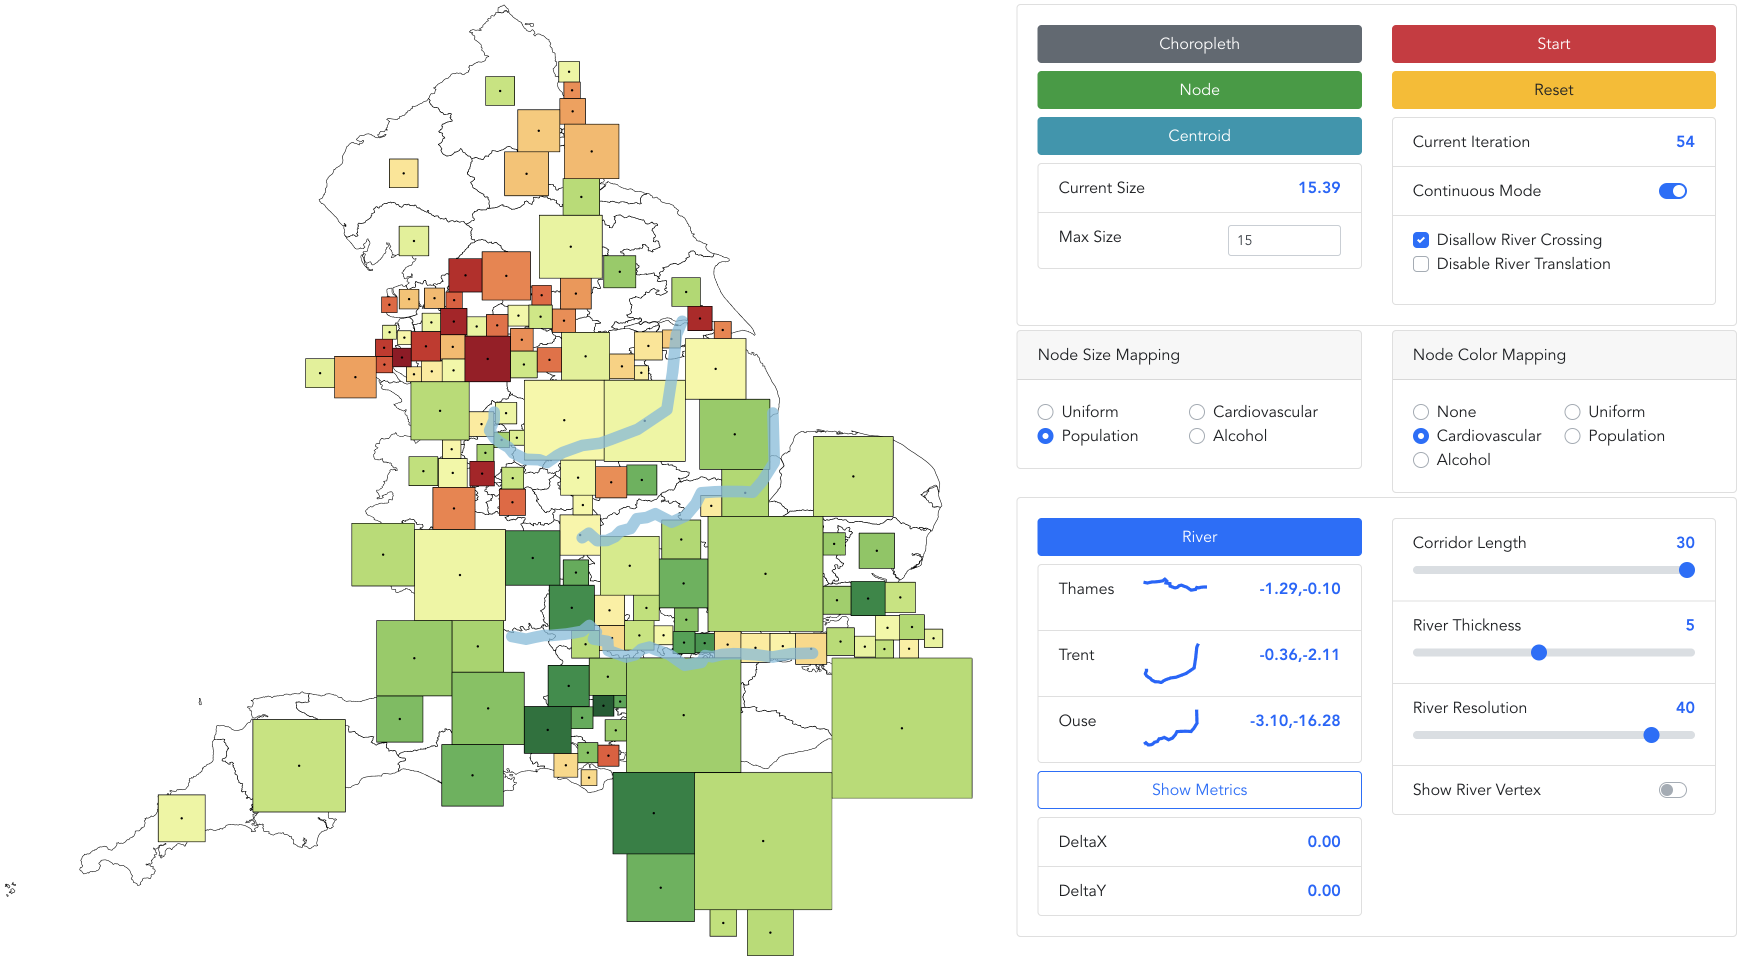
\includegraphics[width=\textwidth,keepaspectratio]{figure/UI.png}
    \caption{A screenshot of the software. User options are provided to adjust the size, color mapping, visibility of nodes and rivers. Other options include the ability to control the overlap removal behavior: rivers can be static or dynamic.}
    \label{fig:overview}
\end{figure*}
}